%% !TeX spellcheck = en_GB

\section{Literature}
\todo{wissen wir bereits, zB aus Powers, dass FLNc KO den Winkel der Z-Scheiben ändert? Ist das valide?}


\section*{AG Fürst Bonn}
We search for supplementary data.
\cite{Holtzhausen2024} Family with hereditary FLNc mutation: Proteome analysis, Protein expression, Obduktion and immunefluorescence-microscopy of the dilated heart tissue. No contraction images.


Ab hier beginnen die Paper in denen Orfanos contributed hat.
\cite{Kley2021}

\subsection*{Rebecca Buschmann - }
\subsubsection*{Allgemeines}

W2711X, es entsteht ein Stoppcodon. "Reflektiert die Situation von Patienten mit Filaminopathie", \cite[p.14]{Unterbusch2017}. Bei heterozygoter Mutation wurde etwa die Hälfte FLNc als trunkiertes FLNc beobachtet. Das spricht für biallelische Expression. Beim Menschen wurden derzeit nur Heterozygote Mutationen beobachtet.
Nach \cite{vanderVen2000gFilamin}, ist die Insertion, die FLNc gegenüber a und b hat für die Lokalisation an den Z-Scheiben verantwortlich.

\textbf{insgesamt geht es in diesem Paper um die Myotubenbildung in Muskelzellen}. Während der Differenzierung ist die EPS angewendet worden und hat womöglich so diesen Prozess, das heißt die Entstehung von Myofibrillen, beeinträchtigt. \todo{als Parameter gibt es hier "nur" EPS protokoll und Bilder. Keine Daten zu Kraft oder Energie oder Calcium. Auch die zeitliche Auflösung ist mit Stundenabständen weniger geeignet}.
\newline 


An Differenzierungstag 6 wurden Zellen nach elektrischer Pulsstimulation (EPS) gestresst.
Stressprotokoll mit 1mm dicken, 20mm voneinander entfernten Elektroden.
\begin{table}[h]
\centering
\begin{tabular}{|c|c|c|}
\hline
Zeitpunkt & Dauer & Frequenz \\
\hline
0 & 5 Sekunden& 15 Hz\\
\hline
0+3h & 60 Sekunden & - \\
\hline
0+6h & 10 Sekunden & 1 Hz \\
\hline
0+9h & 60 Sekunden & - \\
\hline
\end{tabular}


\end{table}

Auf S.35 \cite{Unterbusch2017} findet sich eine Abbildung mit gefärbten Bildern der Zellen an den Differenzierungstagen (0,2,4,6).
Es konnte gezeigt werden, dass die Zellen zum Zeitpunkt der Fixierung an Tag 6 der

Differenzierung noch nicht gut differenziert waren, da durch die Färbung von Filamin C kein Z-

Bandenmuster zu erkennen war (Abbildung 3.12 A und D).

Ist das ein Problem? Schließlich fand an Tag 6 das EPS statt. Oder war das nur : Es konnte gezeigt werden, dass die Zellen zum Zeitpunkt der Fixierung an Tag 6 der
Differenzierung noch nicht gut differenziert waren, da durch die Färbung von Filamin C kein Z-
Bandenmuster zu erkennen war (Abbildung 3.12 A und D). p.53?

weiter p.60: Bisher unveröffentliche Daten (Dr. Julia
Schuld, persönliche Kommunikation) konnten zeigen, dass in homozygoten W2711X
Gewebeschnitten, trunkiertes Filamin C vorwiegend in MTJ lokalisiert zu sein scheint und
vermutlich nicht an der Z-Scheibe.
\textbf{Insbesondere} ist an diesen Daten kein Energieumsatz beobachtbar. Ja, die Zellen wurden durch EPS stimuliert. Aber es gibt keine Daten zu Verkürzungen der Zellen oder gemessenen Kräften. Wir bekommen die Zellen also nur in "passiver" Originallänge. 

\subsection*{Zac Orfanos - breaking Sarcomeres}
\textbf{hier gibt es imaging während contractions}. "Lesions stretch during contraction". Lesions: " we used electrical pulse stimulation (EPS) to simulate exercise in C2C12 myotubes, combined with live microscopy" \cite{orfanos2025}.
\textbf{FLNc only EGFP colorored. No KO.} C2C12 cells. Bilder und damage protokoll. Soleus muscle of a mice. \textbf{live cell imaging}? Contraction was photographed? EPS is similar to Mouse treadmill exercise. (IS EPS also similar to heartbeat in a FLNc KO cell?).
\todo{Wie sind diese Bilder klassifiziert? Welche sind die during contraction Bilder?}

Spannend: Hier wurde also FLNc als Marker von Lesions benutzt. Dieser hat wohl etwas damit zu tuen. Dort wo Lesions sind, sind Sarokmere nicht kontraktil sondern werden passiv geweitet. Ist es möglich, dass in FLNc KO mehr lesions sind und dies häufiger passiert?

\subsection*{Alex Quinn}
Ischämie, das ist für Marianne.
Data on harddrive: Sarcomere lenghts as .txt files. \newline 
Fluorescence as .csv files.
Is there a protocol for these data?



\subsection*{Yvonne Leber}
Sind die einzigen Daten in Cardiomyozyten.
Ist hier das Paper zu den Bildern aus dem AG Fuerst Ordner? \newline 
Keine live contraction Bilder, kein KO.

FLNc rekruitiert auch bei gestoppter Proteinbiosynthese zu den lesions.
\subsection*{Fuerst}
Es gibt Bilder in einem Protokoll zu 0h, 1h, 3h, 5h. Damage, Twitch und unpaced. Gibt es hierzu ein Protokoll?


\subsection*{Timmermann ePub}
\subsection*{Powers - subcellular remodeling}
Tolles paper. Force legth shortening in single cardiomyocytes.
\todo{haben wir diese Daten?}


\subsection*{Fuerst}
Finde kein Protokoll zu den Daten. Bzw. keine Klassifikation der Bilder. Was ist was? Weiterhin hier auch keine Kraftmessung.




\begin{table}[h]
\centering
\begin{tabular}{|l|c|c|c|c|l|}
\hline
Source & FLNc KO vs. WT & EPS/Dmg. Pro & Immuno Images & \makecell{Contr. (CI) \\ or Force (F)} & Commentary \\
\hline
Orfanos & No & Yes & yes & \textbf{C Images}& \makecell{Lesions \\ stretch during contraction } \\
\hline
Unterbusch & yes & yes & yes & no & myotube formation. Alignment und Z-disk struktur. Nicht contraction modeling. \\
\hline
Alex Quinn & ? & ? & ? & ? & Protokoll?\\
\hline
Leber & no & "yes" & yes & no & FLNc as repair\\
\hline
Powers & yes & "yes" & yes & yes & transcriptom and proteom \\
\hline
\end{tabular}
\caption{Data resolution of different sources}
\label{tab:data_resolution}
\end{table}


\todo{Dondl treffen mit Viv anfragen nächste Woche. Montag ab 16h möglich? Mittwoch 3-5. Ansonsten Woche drauf.}
\todo{Powers Open source daten? Publikationen? Website. UW -> joe powers -> open source daten als supplement?}
\todo{calcium ins modell ijf inkorporieren}
\todo{hat Fuerst/Orfanos Videos von kontrahierendem KO}
\todo{Fuerst Ordner EPS protokoll? Welcher stress wurde auf die Daten.}
\todo{orfanos mehr Publikationen? Vielleicht gibt es noch eine zu der die Daten passen?}
\todo{Caspar: du fängst an mit den Videos von Zac.}
\todo{Unterbusch: kann man EPS Protokoll mit FLNc KO vergleichen in der Wirkung auf die Kraftentwicklung?}
\todo{Paper von Orfanos auf AG Fuerst website durchlesen. Auch die beiden Paper (nicht unbedingt von Orfanos von 2025 durchlesen}
\todo{wie verhalten sich Lesions unter contraction in FLNc deficienten zellen anders, als in FLNc WT zellen? Lassen Sie sich }

\listoftodos

\begin{figure}[ht]
\centering
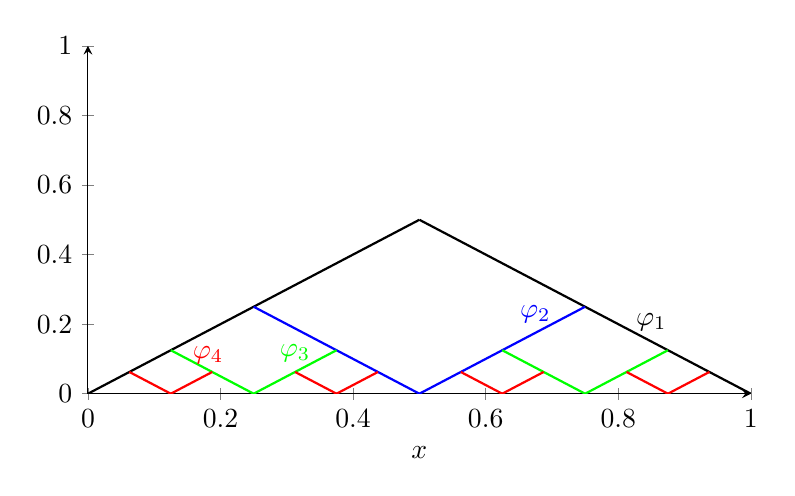
\begin{tikzpicture}
    \begin{axis}[
        width=10cm,
        height=6cm,
        xmin=0, xmax=1,
        ymin=0, ymax=1,
        axis lines=left,
        xlabel={$x$},
        %ylabel={$x$},
        samples=200
    ]
%varphi_1
    % Part 1: f(x) = x on [0, 0.5]
    \addplot[
        domain=0:0.5,
        thick
    ] {x};

    % Part 2: f(x) = 1 - x on [0.5, 1]
    \addplot[
        domain=0.5:1,
        thick
    ] {1 - x}
		node[pos=0.7, above] {$\varphi_1$};

%varphi_2
	%Part 1
	\addplot[
        domain=0.25:0.5,
        thick, blue
    ] {0.5 - x};

	%Part 2
	 \addplot[
        domain=0.5:0.75,
        thick, blue
    ] {-0.5 + x}
		node[pos=0.7, above] {$\varphi_2$};

%varphi_3
	\addplot[
        domain=0.125:0.25,
        thick, green
    ] {0.25 - x};

	 \addplot[
        domain=0.25:0.375,
        thick, green
    ] {-0.25 + x}
		node[pos=0.5, above] {$\varphi_3$};

	\addplot[
        domain=0.625:0.75,
        thick, green
    ] {0.75 - x};

	 \addplot[
        domain=0.75:0.875,
        thick, green
    ] {-0.75 + x};

%varphi_4
	\addplot[
        domain=0.0625:0.125,
        thick, red
    ] {0.125 - x};

	 \addplot[
        domain=0.125:0.1875,
        thick, red
    ] {-0.125 + x}
		node[pos=0.9, above] {$\varphi_4$};

	\addplot[
        domain=0.3125:0.375,
        thick, red
    ] {0.375 - x};

	 \addplot[
        domain=0.375:0.4375,
        thick, red
    ] {-0.375 + x};

	\addplot[
        domain=0.5625:0.625,
        thick, red
    ] {0.625 - x};

	 \addplot[
        domain=0.625:0.6875,
        thick, red
    ] {-0.625 + x};

	\addplot[
        domain=0.8125:0.875,
        thick, red
    ] {0.875 - x};

	 \addplot[
        domain=0.875:0.9375,
        thick, red
    ] {-0.875 + x};
    \end{axis}
\end{tikzpicture}
\caption{Many Lipschitz a.e. solutions. \label{FigureLipschitz}}
\end{figure}
